\documentclass[12pt]{exam}

\newcommand{\ds}{\ensuremath{\displaystyle}}

\usepackage{amsmath,amsfonts, amsthm}
\usepackage{multicol}
\usepackage{multirow}
\usepackage{harpoon}
\renewcommand{\arraystretch}{1.5}

\newcommand{\harpvec}[1]{\overrightharp{\ensuremath{\mathbf{#1}}}}
\newcommand{\vect}[1]{\harpvec{#1}}
\newcommand{\<}{\langle}
\renewcommand{\>}{\rangle}

% ref: http://pgfplots.sourceforge.net/gallery.html
% ref: http://tex.stackexchange.com/a/74575/79754
\usepackage{pgfplots}% This uses tikz
\pgfplotsset{compat=newest}% use newest version
\tikzset{LineStyle/.style={smooth, ultra thick, samples=400}}

% \printanswers

\begin{document}

\begin{center}
\fbox{\fbox{\parbox{5.5in}{\centering
MATH 1121 - Fall 2015 - Dr. Clontz - Test 3
}}}
\end{center}
\vspace{0.1in}
\makebox[\textwidth]{
  Name:\enspace\hrulefill\hrulefill\hrulefill\space
  Section: MW 1100 (001) / TR 1530 (002)
}

\vspace{12pt}

\begin{itemize}
  \item This test is worth 250 points toward your overall grade.
        Each problem is labeled with its value toward this total. Points
        earned beyond 250 will be counted as bonus.
  \item On multiple choice problems, you do not need to show your work. No
        partial credit will be given.
  \item On full response problems, show all of your work and give a
        complete solution. When in doubt, don't skip any steps. Partial
        credit will be given at the discretion of the instructor.
  \item This exam is open notes, provided that these notes are completely
        in your own handwriting. The professor may take up notes you use
        with your test and return them after the test is graded.
  \item Calculators are not necessary to solve any questions on the test and
        are not allowed.
        Notes on electronic devices must be approved by the instructor
        prior to the test day (e.g. for accomodations) and should be in
        airplane mode.
  \item Tests submitted after the end of 70 minutes will be deducted 25 points,
        with 25 more points deducted every following minute.
\end{itemize}

\newpage

\noindent
\textbf{Trigonometric function defintions:}
\begin{itemize}
  \item \(\sin\theta = \frac{opp}{hyp}\)
  \item \(\cos\theta = \frac{adj}{hyp}\)
  \item \(\tan\theta = \frac{opp}{adj}=\frac{\sin\theta}{\cos\theta}\)
  \item \(\csc\theta = \frac{hyp}{opp}=\frac{1}{\sin\theta}\)
  \item \(\sec\theta = \frac{hyp}{adj}=\frac{1}{\cos\theta}\)
  \item \(\cot\theta =
    \frac{adj}{opp}=\frac{1}{\tan\theta}=\frac{\cos\theta}{\sin\theta}\)
  \item
Points on the unit circle satisfy \((x,y)=(\cos\theta,\sin\theta)\):
\end{itemize}
\begin{center}
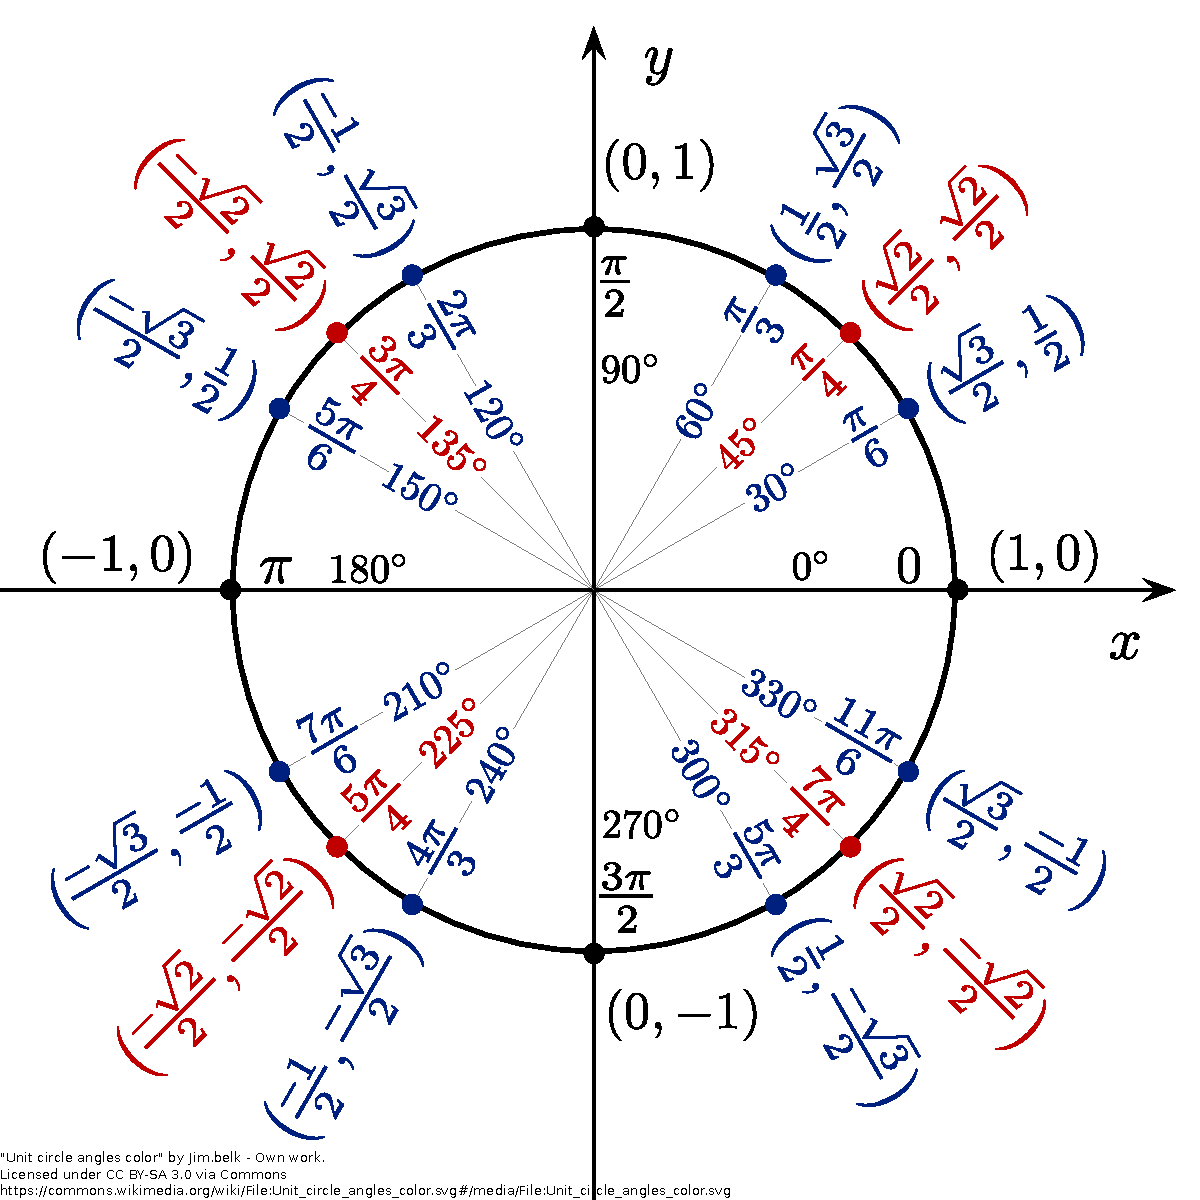
\includegraphics[width=0.7\linewidth]{../unit-circle.pdf}
\end{center}

\noindent
\textbf{Logrithmic Function Definition:}
\begin{itemize}
  \item \(y=\log_b x\) is equivalent to \(x=b^y\)
  \item \(y=\ln x\) is equivalent to \(x=e^y\)
\end{itemize}

\newpage

\noindent
\textbf{Trigonometric/Exponential/Logrithmic Derivatives}

\begin{center}
\begin{tabular}{c|c}
  \(f(x)\) & \(f'(x)\) \\\hline
  \(\sin\theta\) & \(\cos\theta\) \\
  \(\cos\theta\) & \(-\sin\theta\) \\
  \(\tan\theta\) & \(\sec^2\theta\) \\
  \(\cot\theta\) & \(-\csc^2\theta\) \\
  \(\sec\theta\) & \(\sec\theta\tan\theta\) \\
  \(\csc\theta\) & \(-\csc\theta\cot\theta\) \\
  \(\log_b x\) or \(\log_b|x|\) & \(\frac{1}{x}\log_b e\) \\
  \(\ln x\) or \(\ln|x|\) & \(\frac{1}{x}\) \\
  \(b^x\) & \(b^x\ln b\) \\
  \(e^x\) & \(e^x\)
\end{tabular}
\end{center}

\noindent
\textbf{Trigonometric/Exponential/Logrithmic Integrals}

\begin{center}
\begin{tabular}{c|c}
  \(f(x)\) & \(\int f(x)\,dx\) \\\hline
  \(\cos\theta\) & \(\sin\theta+C\) \\
  \(\sin\theta\) & \(-\cos\theta+C\) \\
  \(\sec^2\theta\) & \(\tan\theta+C\) \\
  \(\csc^2\theta\) & \(-\cot\theta+C\) \\
  \(\sec\theta\tan\theta\) & \(\sec\theta+C\) \\
  \(\csc\theta\cot\theta\) & \(-\csc\theta+C\) \\
  \(\frac{1}{x}\) & \(\ln|x|+C\) \\
  \(e^x\) & \(e^x+C\)
\end{tabular}
\end{center}

% \begin{center}
%   \textbf{Multiple Choice (160 points total)}
% \end{center}

% \begin{questions}

% \setcounter{question}{0}

% \question[20]
% Evaluate \(\ds\lim_{x\to 2}\frac{4x^2-8x}{x-2}\).

% \begin{checkboxes}
%   \choice \(\ds\frac{0}{0}\)
%   \choice \(8x\)
%   \choice \(8\)
%   \choice \(0\)
%   \choice None of these.
% \end{checkboxes}

% \vfill

% \question[20]
% Differentiate \(y=4x^3-2x^4+7x-3\).

% \begin{checkboxes}
%   \choice \(y'=3x^4-4x^2+x\)
%   \choice \(y'=12x^2-8x^3+7\)
%   \choice \(y'=8x^7-21x\)
%   \choice \(y'=6x^3-8x^4+7x-3\)
%   \choice None of these.
% \end{checkboxes}

% \vfill

% \question[20]
% Find a formula for the velocity \(v\) of an object whose position \(s\) is
% given by the formula \(s=7+4t-t^3\) for a given time \(t\).

% \begin{checkboxes}
%   \choice \(v=7-3t^2\)
%   \choice \(v=4-3t^2\)
%   \choice \(v=7t^3\)
%   \choice \(v=28-t^2\)
%   \choice None of these.
% \end{checkboxes}

% \vfill
% \newpage

% \question[20]
% Which of the below choices is the (unsimplified) derivative of\\
% \(f(x)=(3x-2)(4x^2+3)\)?

% \begin{checkboxes}
%   \choice \(f'(x)=(4x^2+3)(3)+(3x-2)(8x)\)
%   \choice \(f'(x)=(3)(8x)\)
%   \choice \(f'(x)=(3x-2)(3)+(4x^2+3)(8x)\)
%   \choice \(f'(x)=(24x)(3x-4x^2)\)
%   \choice None of these.
% \end{checkboxes}

% \vfill

% \question[20]
% Which of the below choices is the (unsimplified) derivative of\\
% \(\ds f(x)=\frac{3x^3-x}{2x^2-5x+4}\)?

% \begin{checkboxes}
%   \choice \(\ds f'(x)=\frac{(3x^3-x)(2x^2-5x+4)-(9x^2-1)(4x-5)}{(3x^3-x)^2}\)
%   \choice \(\ds f'(x)=\frac{(2x^2-5x+4)(9x^2)-(3x^3-x)(4x-5)}{(3x^3-x)^2(2x^2-5x+4)^2}\)
%   \choice \(\ds f'(x)=\frac{(3x^3-x)(4x^2-5)-(2x^2-5x+4)(27x-1)}{(3x^3-x)^2}\)
%   \choice \(\ds f'(x)=\frac{(2x^2-5x+4)(9x^2-1)-(3x^3-x)(4x-5)}{(2x^2-5x+4)^2}\)
%   \choice None of these.
% \end{checkboxes}

% \vfill
% \newpage

% \question[20]
% Which of the below choices is equal to \(\frac{dy}{dx}\) given \(y=(2x-3)^3\)?

% \begin{checkboxes}
%   \choice \(6(4x^2-12x+9)\)
%   \choice \(8x^3-36x^2+54x-27\)
%   \choice \(\ds\frac{3}{(2x-3)^2}\)
%   \choice \(8(2x^2-3x)^2\)
%   \choice None of these.
% \end{checkboxes}

% \vfill

% \question[20]
% Which of the below choices is equal to \(\frac{dy}{dx}\) at the point
% \((x,y)=(2,0)\) for the equation \(3xy-y^3=2-x\) implicitly defining \(y\)
% as a function of \(x\)?

% \begin{checkboxes}
%   \choice \(3\)
%   \choice \(0\)
%   \choice \(\frac{2}{7}\)
%   \choice \(-\frac{1}{6}\)
%   \choice None of these.
% \end{checkboxes}

% \vfill

% \question[20]
% Exactly which higher order derivatives of \(f(x)=2x-4x^3+7\) are the zero function?

% \begin{checkboxes}
%   \choice \(f^{(n)}(x)=0\) for all \(n\geq 2\)
%   \choice \(f^{(n)}(x)=0\) for all \(n\geq 3\)
%   \choice \(f^{(n)}(x)=0\) for all \(n\geq 4\)
%   \choice \(f^{(n)}(x)=0\) for all \(n\geq 5\)
%   \choice None of these.
% \end{checkboxes}

% \vfill


% \end{questions}




% \newpage



% \begin{center}
%   \textbf{Full Response (100 points total)}
% \end{center}

% \begin{questions}

% \setcounter{question}{8}

% \question[20]
%   Show how to evaluate \(\ds\lim_{x\to\infty}\frac{6x^2}{2-3x^2}=-2\).
%   {\small (Hint: remember that \(\ds\lim_{x\to\pm\infty}\frac{a}{x^p}=0\) for
%   constant numbers \(a\) and positive constant numbers \(p\).)}

% \newpage

% \question[20]
%   Prove using the limit definition
%     \[
%       f'(x) = \lim_{\Delta x\to 0}\frac{f(x+\Delta x)-f(x)}{\Delta x}
%     \]
%   (what the book calls the ``delta-process'') that the derivative of
%   \[f(x)=\frac{2}{1-x}\] is \[f'(x)=\frac{2}{(1-x)^2}\] (No credit will
%   be given for using shortcuts like the quotient rule or chain rule.)

% \newpage

% \question[20]
%   The formula for the volume of water in a conical tank whose point has
%   an angle of \(90^\circ\) is given by \(V=\frac{1}{3}\pi h^3\), where
%   \(h\) is the height of water in the tank. Find the rate of change of the
%   water's volume with respect to the height of the water when the water
%   is \(2\) units high. (You should leave your answer in terms of the
%   constant \(\pi\).)

% \newpage

% \question[20]
%   Find the derivative of \(y=\frac{4}{\sqrt{1-3x}}\). For full credit,
%   write the derivative as a simplified fraction with denominator \((1-3x)^{3/2}\).

% \newpage

% \question[20]
%   Using the methods of chapter 2, we can show that the circle with
%   center \((3,4)\) and radius \(5\) has the equation
%   \((x-3)^2+(y-4)^2=25\). Use this equation to prove that the slope
%   of the line tangent to this circle at the origin \((0,0)\) is
%   \(-\frac{3}{4}\).

% \end{questions}

\end{document}